\subsection{Overview}


\subsection{Component view}


\subsection{Deployment view}


\subsection{Runtime view}


\subsection{Component interfaces}


\subsection{Selected architectural styles and patters}

\subsubsection{Architecture patterns}
\begin{itemize}
    \item 
    \textbf{Three tier architecture:} As already mentioned, the SafeStreets system is divided into three tiers: Presentation, Business Logic and Persistence tier.
    \item
    \textbf{Client-Server architecture:} Computing model in which the server hosts, delivers and manages most of the resources and services that are consumed by the clients.

    \begin{figure}[H]
    \centering
    \fbox{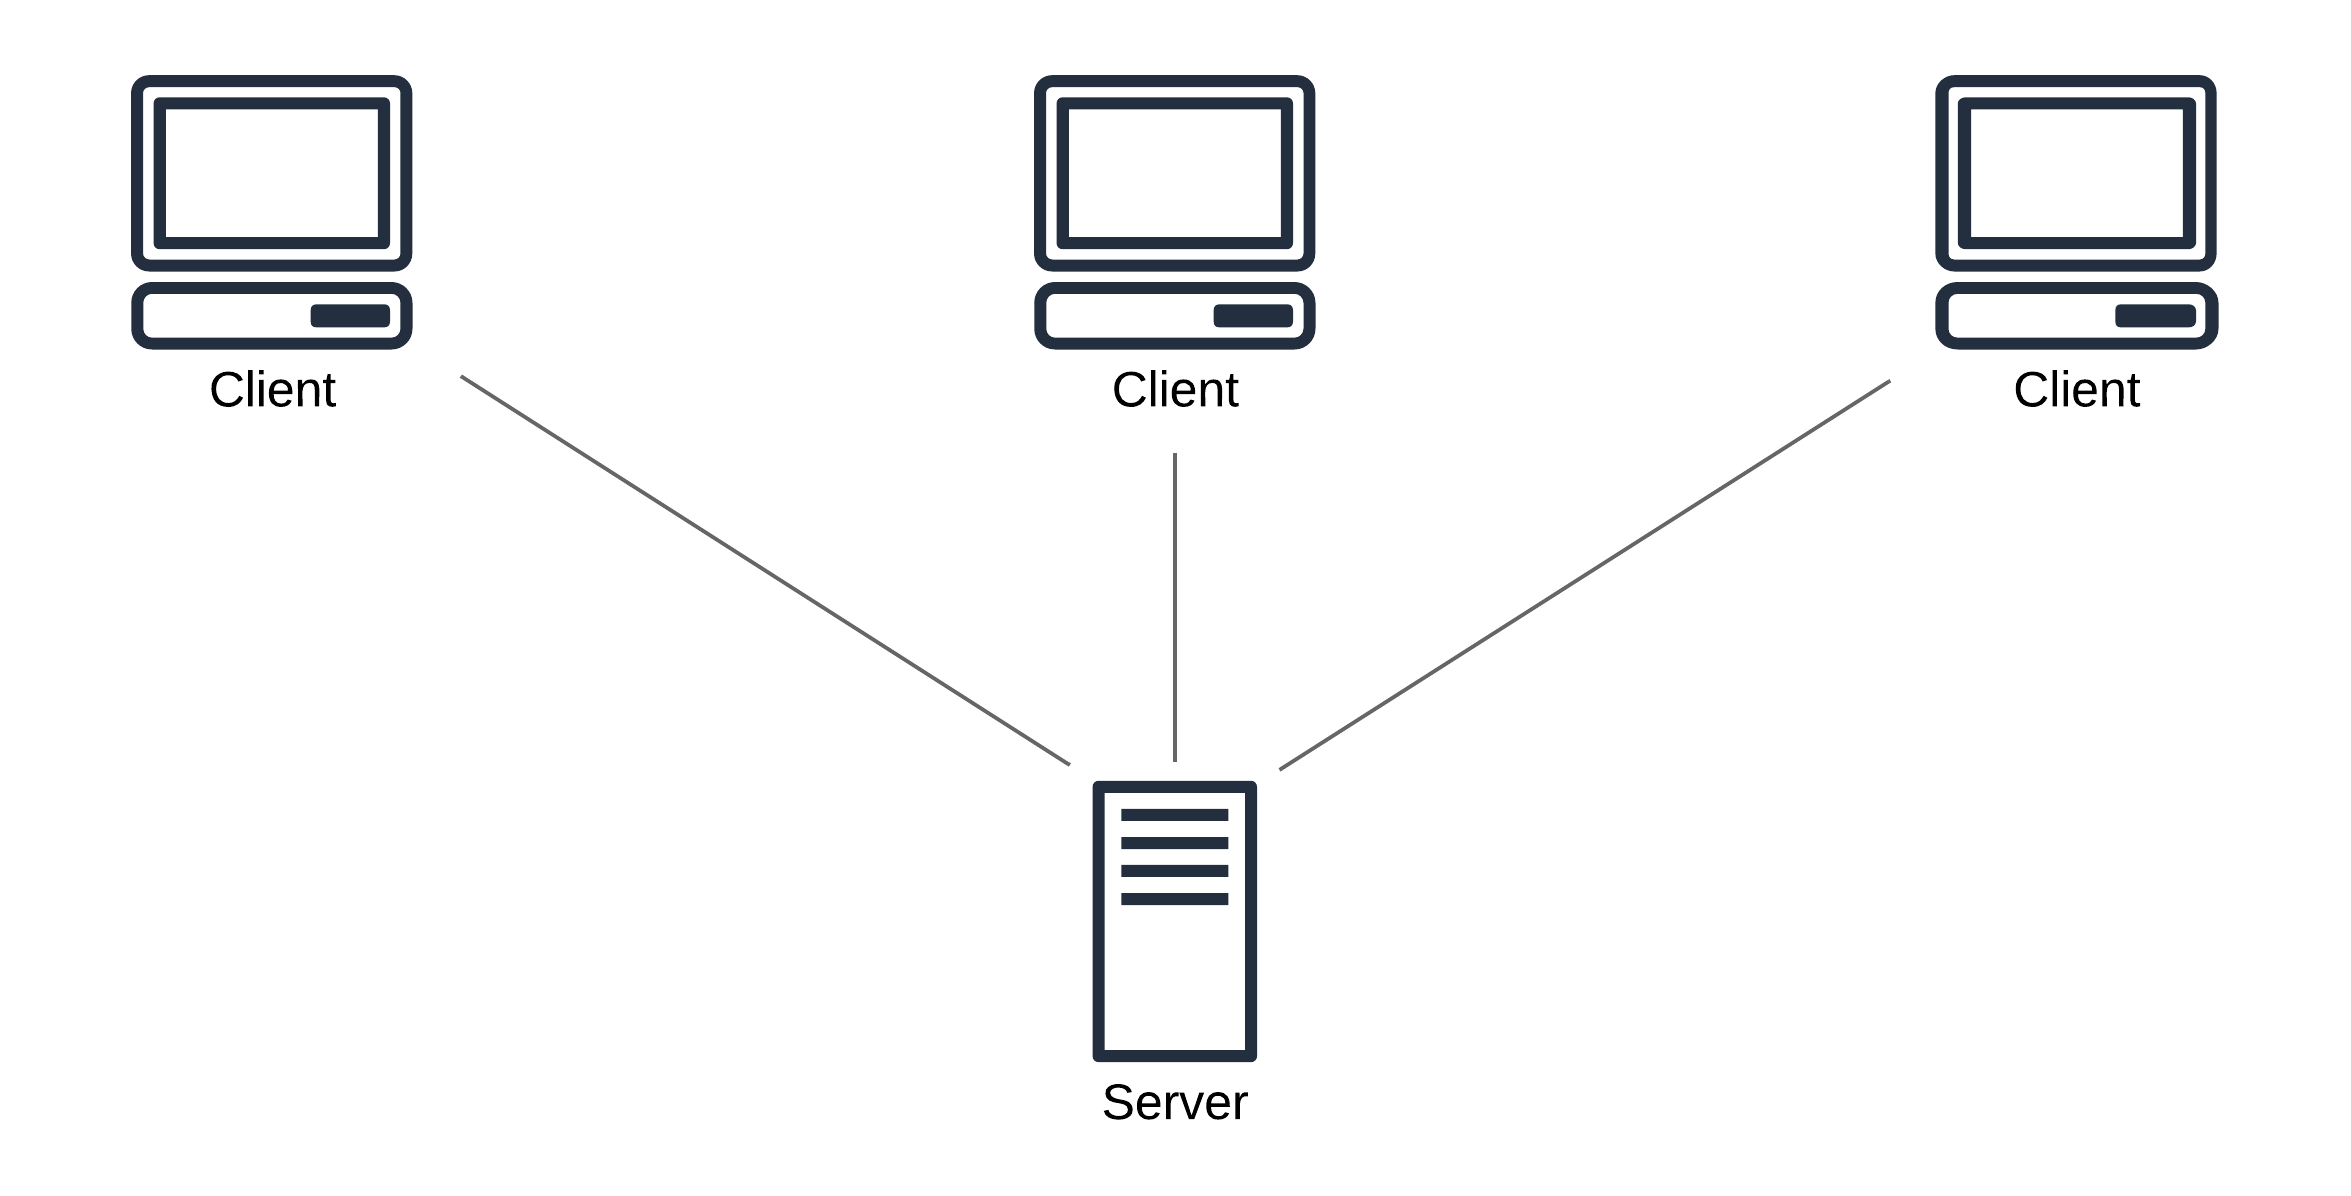
\includegraphics[width=0.8\textwidth]{Images/client-server-architecture.png}}
    \caption{\label{fig:api-usage}Client-Server architecture.}
    \end{figure}

    The mobile devices running the application are the clients, which interact with the business logic tier (Application server); it is here that the heavy computation of the system is done. The “Thin Client Server architecture” can also be referenced.
\end{itemize}

\subsubsection{Design patterns}
\begin{itemize}
    \item
    \textbf{Model-View-Controller:} Divides the program logic into three interconnected elements.\\
        \hspace*{3ex}-\hspace*{2ex}Model: Central component. Manages the data, logic and rules of the application.\\
        \hspace*{3ex}-\hspace*{2ex}View: Visual representation of the model.\\
        \hspace*{3ex}-\hspace*{2ex}Controller: Accepts inputs and converts it to commands for the model or view.

    \begin{figure}[H]
    \centering
    \fbox{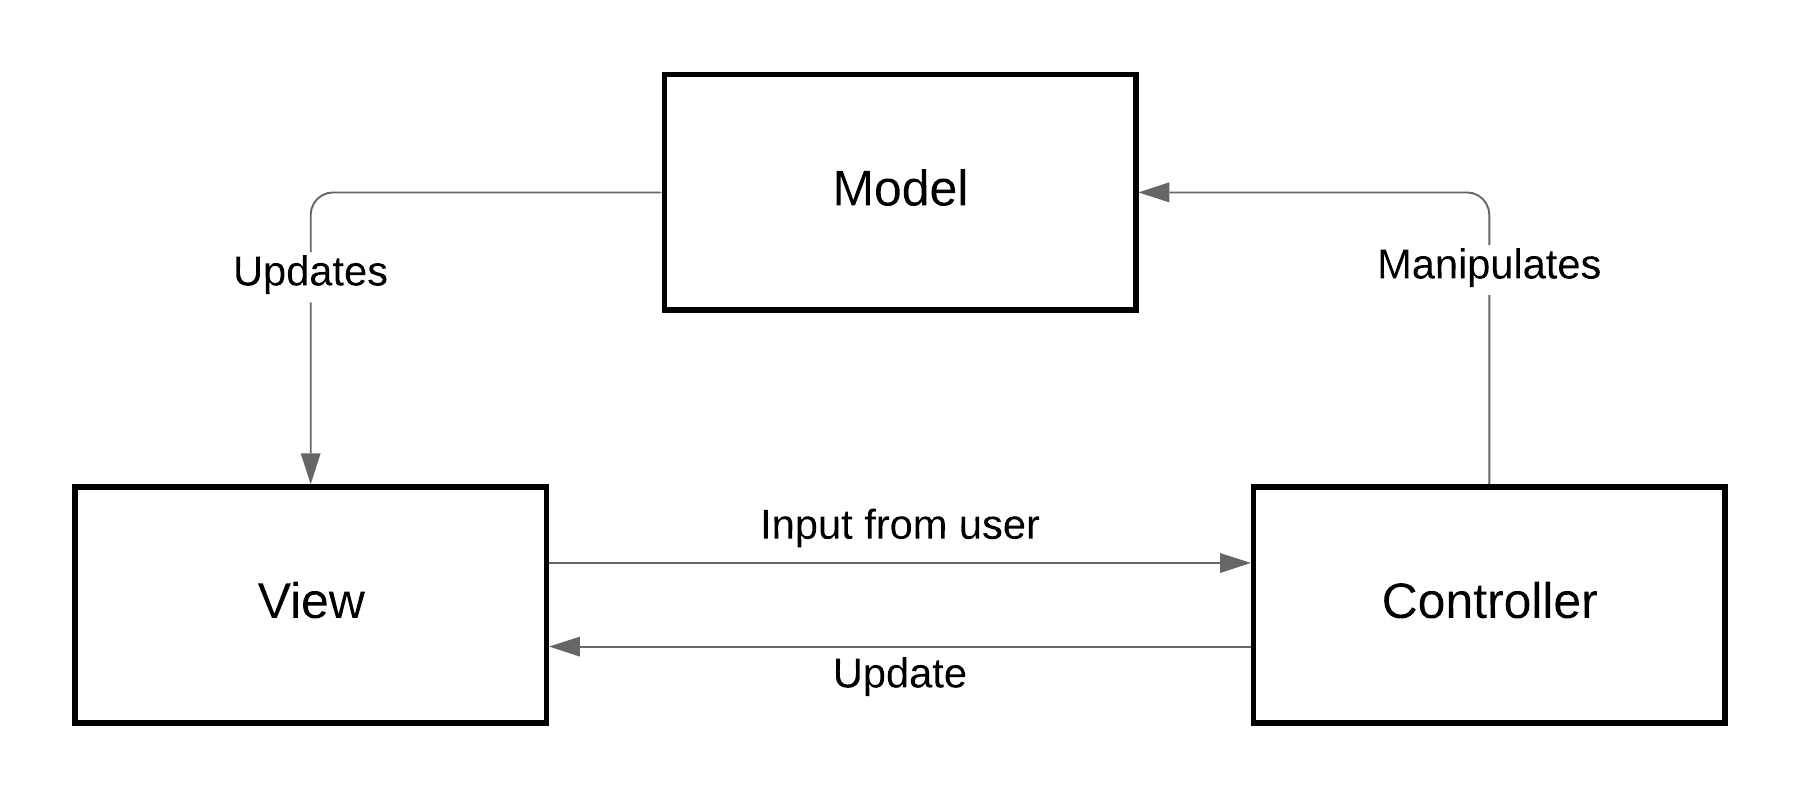
\includegraphics[width=0.8\textwidth]{Images/mvc-pattern.png}}
    \caption{\label{fig:api-usage}Model View Controller pattern.}
    \end{figure}

    This pattern is used in the development of the mobile application, which is the part of the system the user directly interacts with.

    \item
    \textbf{Facade pattern:} Provides a simple interface to a larger body of code. This is used in the backend to expose the API to external users. The router component acts as the facade, interacting with the lower level components and exposing the appropriate endpoints.

    \begin{figure}[H]
    \centering
    \fbox{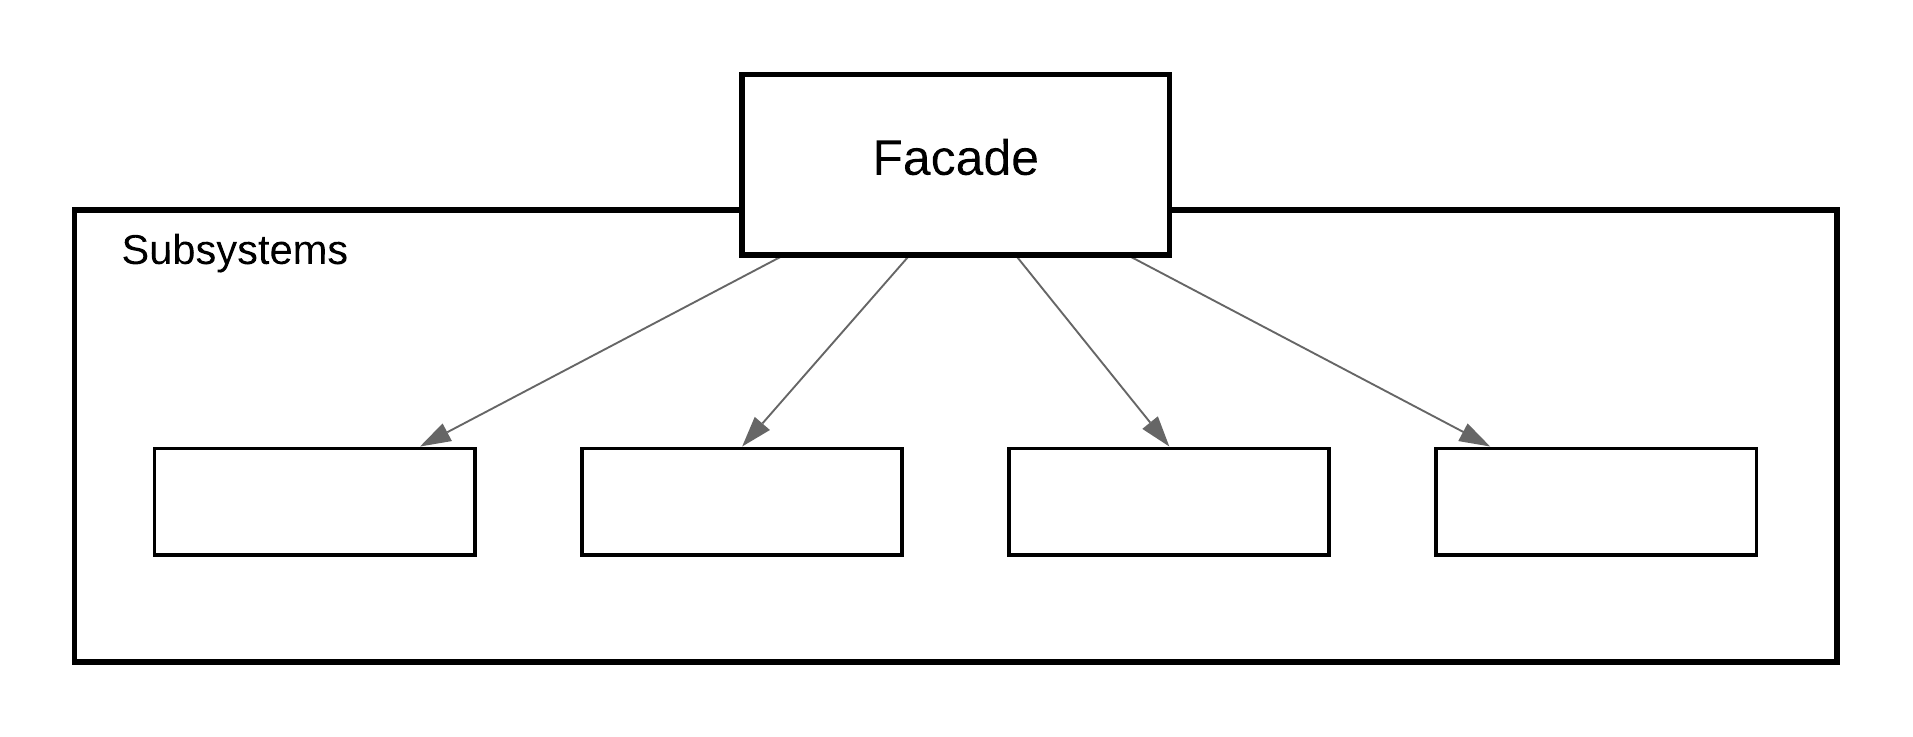
\includegraphics[width=0.8\textwidth]{Images/facade-pattern.png}}
    \caption{\label{fig:api-usage}Facade pattern.}
    \end{figure}

    \item
    \textbf{Dependency injection pattern:} A technique whereby one object supplies the dependencies of another object.\\
    Utilized in the backend to solve the dependencies between services.



\end{itemize}

\subsection{Other desing decisions}